\documentclass[a4paper,12pt]{report}
\usepackage[spanish]{babel}   % español
\usepackage[utf8]{inputenc}   % acentos sin codigo
\usepackage{graphicx}         % graficos
\usepackage[document]{ragged2e}
\usepackage{fancyhdr}		%encabezados y pies de pagina
\usepackage[right=2.54cm,left=3.04cm,top=2.54cm,bottom=2.54cm,headsep=0.5cm,footskip=0.8cm]{geometry}
\usepackage{natbib}			% para referencias bibliograficas
\usepackage{url}			% referencias bibliograficas WEB
\usepackage{enumerate}		% viñetas y numeracion
\usepackage{pdflscape}		% paginas en horizontal
\usepackage{multirow}		% para tablas
\usepackage{longtable}		% para tablas largas
\usepackage{lineno}			% para numerar las lineas
\usepackage{subcaption}		% para imagene multiples


% editando encabezados
\lhead[]{}
\chead[]{}
\rhead[]{}
\renewcommand{\headrulewidth}{0pt}
\fancypagestyle{plain}{
	\fancyhead[L]{}
	\fancyhead[C]{}
	\fancyhead[R]{}
	\renewcommand{\headrulewidth}{0pt}
}

\pagestyle{fancy}

% nivel que se numera y aparece en el indice
\setcounter{secnumdepth}{3}
\setcounter{tocdepth}{3}

% quitar el 0.
\renewcommand\thesection{\arabic{section}}

%=========================
%INICIO del plan de tesis
%=========================

\begin{document}

% INICIO - Caratula de plan de tesis
\begin{titlepage}
\begin{center}

%INICIO - Logo
\begin{figure}[htb]
	\begin{center}
	
\includegraphics[width=6cm]{imagenes/logo.png}
	\end{center}
\end{figure}
%FIN - Logo
% INICIO - datos de la Universidad
\uppercase{universidad nacional de san antonio abad del cusco}
% FIN - datos de la Universidad, Facultad y Escuela


%INICIO - Titulo de la tesis
\vspace*{0.40in}
%\begin{large}
PLAN DE TESIS
%\end{large}


\rule[2mm]{14.5cm}{1mm}%linea de separación

\uppercase{\textbf{``Título del Proyecto de tesis"}}

\rule[0.5mm]{14.5cm}{1mm}%linea de separación
\vspace*{0.3in}
\end{center}
%INICIO - Titulo de la tesis

%INICIO - datos del motivo de plan tesis, autor, asesor
\vspace*{0.3in}
\begin{flushleft}
	\hspace{4.0cm} Para optar al título profesional de:\\
	\hspace{4.5cm} \uppercase{Ingeniero informático y de sistemas}

	\hspace{4.0cm} Presentado por:\\
	\hspace{4.5cm} \uppercase{ Denis Angel Nahuamel Sarce}

	\hspace{4.0cm} Asesor:\\
	\hspace{4.5cm} \uppercase{Dr. Rony Villafuerte Serna}
\end{flushleft}
% FIN - datos del motivo de tesis, autor, asesor


%INICIO - lugar y añor de desarrollo de tesis
\vspace*{2.0in}
\begin{center}
Perú, Enero del 2019

%INICIO - datos de facultad y escuela
\uppercase{\small{escuela profesional de ingeniería informática y de sistemas}}
\scriptsize{\uppercase{facultad de ingeniería eléctrica, electrónica, informática y mecánica}}
%FIN - datos de  facultad y escuela
\end{center}
%FIN - lugar y añor de desarrollo de tesis

\end{titlepage}		
% FIN - Caratula de plan de tesis

\begin{abstract}
Debe contener el tema de la investigación, su importancia, sus objetivos propuestos, estrategias metodológicas, y posibles aplicaciones. Debe ser redactado en un solo párrafo y no contener espacios entre lineas, ni sangría máximo 400 palabras.

\noindent
\textbf{Palabras clave}: palabra 1, palabra 2, palabra 3.
\end{abstract}

%indices
\newpage
% \pdfbookmark{\contentsname}
\tableofcontents 

\newpage
\listoffigures

\newpage
\renewcommand{\listtablename}{Índice de Tablas} %cambiar el nombre del indice de cuadros a indice de tablas
\listoftables

% Numerar las lineas para efectos de revisión por parte del asesor
% Este comando se comentara para la impresión oficial
\linenumbers
\newpage
\section{Antecedentes}
% Apellido letra del Nombre (Juan Perez), año, titulo del trabajo, institucion, pais
Perez J, (2013),\textit{Nombre del proyecto}, Institución donde se desarrollo, País.

\noindent
\textbf{Conclusiones:}
\begin{itemize}
	\item objetivo 1.
	\item objetivo 1.
	\item objetivo N.
\end{itemize}

\noindent
\textbf{Comentario:} Aquí se expone de que manera nos servirá este proyecto, si es para continuar la investigación, sacar marco teórico, o algún algoritmo o pruebas consideradas útiles para nuestro trabajo futuro.

\section{Problema de Investigación}
\section{Objetivos}
\subsection{Objetivo General}
\subsection{Objetivo Especifico}
\begin{itemize}
	\item Indicar cuál sería el objetivo especifico X.
	\item Indicar cuál sería el objetivo especifico Y.
	\item Indicar cuál sería el objetivo especifico Z.
\end{itemize}

\section{Justificación}
Se justifica en párrafos cada objetivo especifico respondiendo a la pregunta ¿Para que --Objetivo específico 1--?

\section{Hipótesis}
(opcional) según tipo de investigación seleccionado
Según tema de investigación puede ser:
\begin{itemize}
\item explorativa: NO tiene hipótesis.
\item descriptiva: NO tiene hipótesis.
\item correlacional, SI tiene hipótesis, tiene estudio de variables, análisis de resultados y discusión.
\item explicativa: SI tiene hipótesis,, tiene estudio de variables, análisis de resultados y discusión.
\end{itemize}

\section{Alcances y limitaciones}
\subsection{Alcances}
Indicar hasta donde nos proponemos llegar con el trabajo de investigación, comparación de algoritmos, mejora de los mismo, implementación de un sistema o creación de un prototipo, lo que se requiera.
\subsection{Limitaciones}
Enmarcar detalladamente el trabajo de investigación a nivel temporal y espacial.

\section{Marco Teórico}
\subsection{sobre el tema uno}
hablamos un poco sobre el tema en cuestión como para que el lector se entere de que va el trabajo a desarrollar y nunca olvidar las referencia de donde las sacamos, pueden ser libros físico o libros electrónicos como también contenido de paginas web, o papers \citep{Larranaga}.
\subsection{sobre el tema dos}
hablamos un poco sobre el tema en cuestión como para que el lector se entere de que va el trabajo a desarrollar y nunca olvidar las referencia de donde las sacamos, pueden ser libros físico o libros electrónicos como también contenido de paginas web, o papers\citep{herz01}.
\subsubsection{algun tema mas}
esto si por allí queremos dar mas énfasis a algún tema pero no hay indentado esto queda solo allí, y ojo  ver figura \ref{fig:ojo01} todo con sus referencia bibliográficas estilo APA

%% LLAMADAS A FIGURAS
\begin{figure}[htb]
	\centering	
	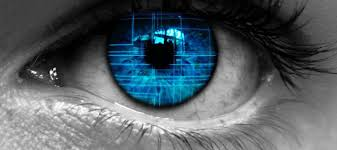
\includegraphics[scale=0.5]{imagenes/ojo.jpg}
	\caption{Ojo digital.}
	\label{fig:ojo01}
\end{figure}

\subsection{sobre el tema tres}
hablamos un poco ver tabla \ref{tbl:tabla01} sobre el tema en cuestión como para que el lector se entere de que va el trabajo a desarrollar y nunca olvidar las referencia de donde las sacamos, pueden ser libros físico o libros electrónicos como también contenido de paginas web, o papers.

% Please add the following required packages to your document preamble:
% \usepackage{booktabs}
\begin{table}[ht]
\centering
\caption{Descripción del contenido}
\label{tbl:tabla01}
\begin{tabular}{@{}lllll@{}}
\hline
COD  & DESCRIPCIÓN   & CR & HRS & CAT \\ \hline
A123 & Matemática 01 & 2  & 4   & OE  \\
A321 & Algorítmica   & 5  & 4   & OE  \\
A456 & Ensamblador   & 2  & 2   & EE  \\ \hline
\end{tabular}
\end{table}

\subsection{sobre el tema cuatro}
Hablamos un poco sobre el tema en cuestión como para que el lector se entere de que va el trabajo a desarrollar ver imagen \ref{fig:ojo01} y nunca olvidar las referencia de donde las sacamos, pueden ser libros físico o libros electrónicos como también contenido de paginas web, o papers \cite{wikiRed}.

\section{Método de desarrollo}
Aquí hay que elegir cuidadosamente el el tipo de investigación según un único autor para no estar construyendo un método de investigación mezclado, recomiendo usar a \citep{sampieri} , quien define claramente los tipos de investigación en Explorativa, descriptiva, correccional y explicativa; las dos primeras no necesitan de Hipótesis y por ende son las mas recomendadas mientras que las 2 ultimas requieren de Hipótesis y un análisis de variables eso no quiere decir que sean difíciles solo hay que tener mas tiempo.
\section{Resultados}
\section{Contribuciones}
\section{Impacto Social}
\section{Indice Tentativo de proyecto de Tesis}
\section{Cronograma de actividades}
\section{Presupuesto}
\nolinenumbers

\newpage
\addcontentsline{toc}{chapter}{Bibliografía}
\bibliographystyle{apalike}
\renewcommand{\refname}{Bibliografía}  %para cambiar el nombre del bloque por defecto (REFERENCIAS => Bibliografia)
\bibliography{Bibliografia} %nombre del archivo .bib



%FIN plan de tesis
\end{document}